\documentclass[a4paper, 10pt]{article}
    \usepackage[subpreambles=true]{standalone}
    \usepackage[english, american, british]{babel}
    \usepackage[utf8]{inputenc}
    \usepackage[T1]{fontenc}
    \usepackage{hyphenat}
    \hyphenation{Mathe-matik wieder-gewinnen}
    \usepackage{amsmath}
    \usepackage{import}
    \usepackage{tabularx}
    \usepackage{graphicx}
    \usepackage[margin=2cm ]{geometry}

    \title{Einführung in die Softwaretechnik 2018 \\ Sheet 05}
    \author{Maximilian Frühauf}

\begin{document}
\maketitle
\begin{enumerate}
    \item 
    Explain the difference between a closed architecture and an open
    architecture and provide examples. Which design goals are realized by closed and
    open architectures and how? Give examples.
    \vspace{0.5cm}

    Systems architectures decompose the current system into different layers. 

    In a closed architecture an object of a  given layer only uses functionality from the immediate layer below it.
    This results in a high Flexibility of the system because if any layer needs to be replaced,
    only the interface to the layer immediately above needs to be considered. 
    Maintainability is also achieved within this layering because any bugs that occur can be traced back
    to a specific layer and therefor be localized faster, than in an open architecture.

    An example of a closed architecture is the ISO / OSI Model for networked communication. 
    Here the Network Layer only uses functionality in the shape of ethernet frames from the Datalink Layer.
    It then provides it's functionality to the Transport Layer above. 
    \vspace{0.5cm}

    A system can also bes designed as an open architecture, in which an object can call functionality from any
    layer below it in the hierarchy. 
    This results in a higher overall performance of the system because the amount of abstractions 
    that need to be considered when executing a function is lower.

    An example of an open architecture is a watch. In this system the user can interface with the device
    via the watch face and read the time. However it is also possible for him to go one level below the abstraction
    of the watch face and for example change the battery. This requires him to have knowledge of underlying layers 
    of the system.

    \item
    Extend the following UML sequence diagram by modeling the detection of a
    collision and the determination of a winner (use the description of the flow of events in
    the Win Collision scenario in Homework Sheet 04, exercise 3).
    \vspace{0.5cm}

    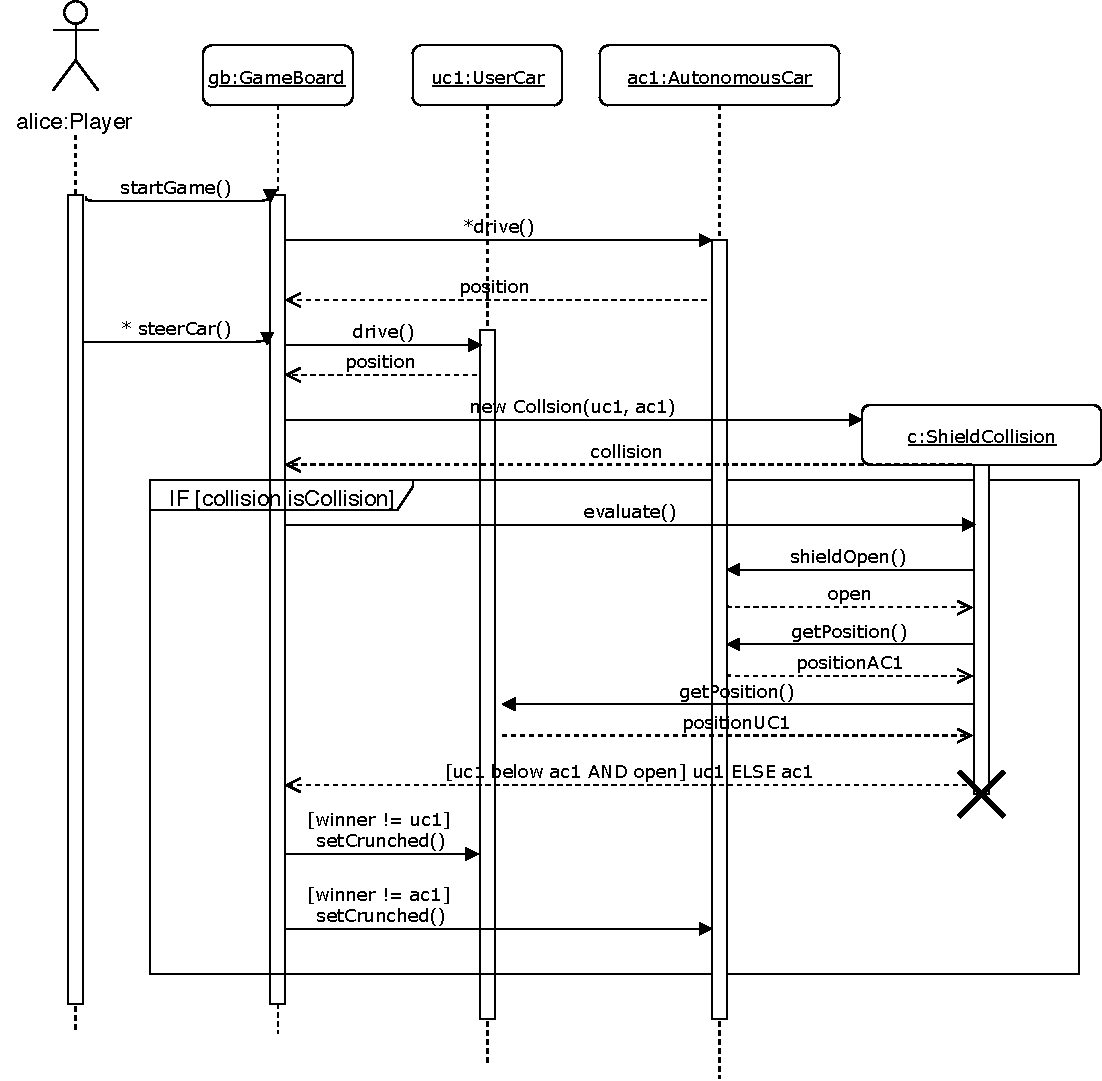
\includegraphics[width=\linewidth]{SequenceDiagram.pdf}

    \item
    Describe the involvement of the stakeholders (client, user, developer) during
    the requirements elicitation activity and discuss their strengths and weaknesses.
    \vspace{0.5cm}

    \begin{itemize}
        \item Client

        The clients goals early in a project during the requirements elicitation phase are 
        low cost, increased productivity, backward compatibility, traceability of requirements,
        Rapid development and Flexibility. These are all goals that interest the client alone and are 
        mostly related to minimizing cost wile maximizing the compatibility of the new system with existing ones.

        This role has the strength to make sure the project is delivered within the layed out schedule and within budgetary
        constraints. It also acts as the mediator between the user and the developer. 
        \item Developer

        The developers goals are a minimum number of errors in the system, modifiability, readability, 
        reusability, adaptability and well defined interfaces.
        These goals focus on making the developed system as easy as possible to change in the future. 
        As well as make it easy to develop the system in a large team. 

        This role has the strength to make sure the project is extensible in the future and can be changed by any 
        developer on the team. It also makes sure that all features are well documented. But it needs the combination of 
        user and client to make sure runtime efficiency is achieved. 
        \item End User

        The end user's goals are an implementation of desired functionality, user-friendliness, usability,
        ease of learning, fault tolerance and robustness.
        These goals focus on the delivered features of the system as well as it's fault tolerance to all kinds of 
        errors.

        This roles strength is a focus on the functional requirements of the system. It also makes sure that 
        the delivered system is usable and solves the desired problems.

        However all of there roles combine the desire to make the system as reliable as possible.
    \end{itemize}
    \item
    Explain how analysis models influence system design issues. Use an
    example from your own experience or Bumpers for each design issue.
    \vspace{0.5cm}

    \begin{itemize}
        \item Nonfunctional Requirements

        Definition of design goals:
        
        The design goals for bumpers are expressed within the original problem statement introduced in lecture 02. 
        They are also listed within the Initial Product backlog.
        \item Functional model 

        Subsystem decomposition:    

        In bumpers the Use Case Diagram describes a first decomposition of the system into different subsystems.
        Each group of the use cases an be defined as a subsystem.

        \item Object model

        Hardware / Software Mapping:

        The UML Class diagram of the bumpers game describes the mapping of the problem statement to objects in an 
        object oriented programming langauge. This process also clarifies if it is required to purpose build a system or 
        use a more generic system available on the market and customize it to the projects needs. In Bumpers it was chosen to 
        use the standard library for any use cases where applicable and implement a custom solution otherwise.
        Here connectivity between the different classes is also defined graphically within the communication diagram.

        Persistent Data Management:

        The persistent data of the bumpers game can be modeled with a Statechart diagram as any state of the 
        entity objects the system is using is displayed here. Therefore if any state needs to persist beyond a single 
        execution of the game it could be saved in a database or on the filesystem. As this is not needed for Bumpers, it 
        does not use a database.

        \item Dynamic model 

        Identification of Concurrency: 
       
        In Bumpers any required concurrent execution of different functions can be modeled with an activity diagram.
        This is shown in the activity diagram from sheet 4 where the collision detection is done in parallel.

        Global Ressource Handling:

        The global ressource handling of Bumpers can be shown in the sequence diagram of for example the collision. 
        Here the access of different methods to the users of the system is modeled by the different objects interacting with
        each other. Messages can only be passed if the corresponding object has the required Access control capabilities.

        Software Control:

        Bumper's Sequence Diagram also shows the design decision of the overall system architecture. Here it can 
        be seen from the passed messages if a monolithic, distributed or event driven design was chosen. 
        \item Hardware / Software mapping

        Boundary Conditions:

        Additional boundary conditions like 
        can also be displayed in the Use Case Diagram. They can 

    \end{itemize}

    \item Explain all of the typical design goal trade-offs introduced in lecture 04, slide
    58, by using your own experience.
    \vspace{0.5cm}

    \begin{itemize}
        \item Functionality vs. Usability
        
        When developing a system there is always the tradeoff between adding more functionality on to it 
        and keeping it usable.
        This tradeoff can be seen within the bumpers game. Here the addition of a shield collision to the 
        game added extra functionality but also made it initially harder for the user to grasp the collision mechanic.
        This is because he needs to understand, that he is required to approach to opposing car from below and 
        can only crunch it if it's shield is currently down.
        These are therefore both design goals that directly impact the user stereotype in the end product.
        \item Cost vs. Robustness

        The tradeoff between cost and robustness is created by the fact that robustness can only be achieved by 
        testing which requires development time. Therefore additional costs are created. 
        This is a tradeoff that was apparent only indirectly to me, when developing a chat client. In the late stages of 
        the project we were short on time and had to skip the amount of error checking we were doing. Therefore the 
        robustness of the final product suffered, as we were unable to catch all of the edge case bugs.
        \item Efficiency vs. Portability

        A tradeoff between efficiency and portability can be best seen early in the development of a project with the 
        choice of the programming language. Here a language like Java that is platform independent has to be compared to 
        one that is initially constrained to a single system like C++. 
        This choice is apparent in the bumpers game as it is written in Java. Here the tradeoff was made as students can 
        use any operating system of their choice. Therefore it needs to be possible to develop Bumpers on all of them,
        which led to the langauge choice of Java. If this was no concern C++ might have also been a valid option.
        \item Rapid development vs. Functionality

        As each feature in a software project takes a certain amount of time to get implemented and tested well enough 
        to be shipped to the client and ultimately the end user a tradeoff between Rapid Development and Functionality has to
        be made.
        This was apparent when developing the chat program, because as we were approaching our deadline we had to cut 
        several of the planned features as we were running out of time. In this situation we focused on a reduced set of features 
        that we were sure on we could deliver on time and with sufficient quality. 
        \item Cost vs. Reusability

        Writing code requires a constant tradeoff between cost in the form of more time spend or reusability of the produced code.
        This was again apparent on the chat project as we chose to make the code as clean and usable as possible to help us move faster in 
        the future when changes were necessary. This also helped us when working on the network communication between multiple clients of the
        programm and the server. Here we were able to design code to handle the communication on the client as well as the 
        server.
        \item Backward Compatibility vs. Readability

        When having to interface with older systems often implementations have to be changed to accommodate them.
        I have personally seen this on a current project for computing the mandelbrot set in C++. Here it's an outside requirement to 
        interface with an old concurrency standard for managing threads which caused several issues during deployment of the application. 
        To still make sure the application is executable on many systems we had to run it in a virtual machine that emulates the older
        environment. This however introduced additional complexity to the system as any developer who want's to execute the programm now 
        has to deal with the virtual machine environment. This therefore also reduced the readability of the application's source code.
    \end{itemize}
\end{enumerate}
\end{document}